%%%%%%%%%%%%%%%%%%%%%%%%%%%%%%%%%%%%%%%%%
% "ModernCV" CV and Cover Letter
% LaTeX Template
% Version 1.11 (19/6/14)
%
% This template has been downloaded from:
% http://www.LaTeXTemplates.com
%
% Original author:
% Xavier Danaux (xdanaux@gmail.com)
%
% License:
% CC BY-NC-SA 3.0 (http://creativecommons.org/licenses/by-nc-sa/3.0/)
%
% Important note:
% This template requires the moderncv.cls and .sty files to be in the same 
% directory as this .tex file. These files provide the resume style and themes 
% used for structuring the document.
%
%%%%%%%%%%%%%%%%%%%%%%%%%%%%%%%%%%%%%%%%%

%----------------------------------------------------------------------------------------
%	PACKAGES AND OTHER DOCUMENT CONFIGURATIONS
%----------------------------------------------------------------------------------------

\documentclass[12pt,a4paper,sans]{moderncv} % Font sizes: 10, 11, or 12; paper sizes: a4paper, letterpaper, a5paper, legalpaper, executivepaper or landscape; font families: sans or roman

\moderncvstyle{banking} % CV theme - options include: 'casual' (default), 'classic', 'oldstyle' and 'banking'
\moderncvcolor{blue} % CV color - options include: 'blue' (default), 'orange', 'green', 'red', 'purple', 'grey' and 'black'

\usepackage[utf8]{inputenc}
\usepackage[T1]{fontenc}
\usepackage{lipsum} % Used for inserting dummy 'Lorem ipsum' text into the template
\usepackage{parcolumns}
\usepackage{comment}
\usepackage{multirow}
\usepackage{eurosym}

\usepackage{xspace}
\newcommand{\fenics}{\textsc{FEniCS}\xspace}
\newcommand{\firedrake}{\textsc{Firedrake}\xspace}

\nopagenumbers 


\usepackage[top=2cm, bottom=2cm, left=2.5cm, right=2.5cm]{geometry} % Reduce document margins
%\setlength{\hintscolumnwidth}{3cm} % Uncomment to change the width of the dates column
%\setlength{\makecvtitlenamewidth}{10cm} % For the 'classic' style, uncomment to adjust the width of the space allocated to your name

\definecolor{color1}{rgb}{0.22,0.45,0.70}% light blue
%----------------------------------------------------------------------------------------
%	NAME AND CONTACT INFORMATION SECTION
%----------------------------------------------------------------------------------------

\firstname{Andrea} % Your first name
\familyname{BRUGNOLI} % Your last name

%% All information in this block is optional, comment out any lines you don't need
%\address{Via Ca' del Frate 7 E}{Negrar (VR), Italy 37024}
%\mobile{(+39) 340 8323361}
%% \phone{(000) 111 1112}
%% \fax{(000) 111 1113}
%\email{brugnoss.ab@gmail.com}
%% \homepage{staff.org.edu/~jsmith}{staff.org.edu/$\sim$jsmith} % The first argument is the url for the clickable link, the second argument is the url displayed in the template - this allows special characters to be displayed such as the tilde in this example
%\extrainfo{Skype contact: brugnoss}
%\photo[70pt][0.4pt]{pictures/Foto_cv} % The first bracket is the picture height, the second is the thickness of the frame around the picture (0pt for no frame)

\AtBeginDocument{\hypersetup{colorlinks=true,
		linkcolor=blue,
		urlcolor=cyan,}}


\patchcmd{\makehead}
{\hfil}
{\hspace*{0.15\textwidth}}
{}
{}
\patchcmd{\makehead}
{\setlength{\makeheaddetailswidth}{0.8\textwidth}}
{\setlength{\makeheaddetailswidth}{0.67\textwidth}}
{}
{}
%\patchcmd{\makehead}
%{\\[2.5em]}
%{\hfil\raisebox{-.7cm}{\framebox{\includegraphics[width=\@photowidth]{\@photo}}}\\[2.5em]}
%{}
%{}

\newcommand*{\httpslink}[2][]{% <=======================================
	\ifthenelse{\equal{#1}{}}%
	{\href{https://#2}{#2}}%
	{\href{https://#2}{#1}}}

\newcommand*{\googlescholarsocialsymbol}  {
\includegraphics[width=0.27cm]{logo_scholar}~} % <===================
\newcommand*{\researchgatesocialsymbol}  {
\includegraphics[width=0.27cm]{logo_researchgate}~} % <===================

\makeatletter
\RenewDocumentCommand{\social}{O{}O{}m}{%
	\ifthenelse{\equal{#2}{}}%
	{ 
		\ifthenelse{\equal{#1}{linkedin}}{\collectionadd[linkedin]{socials}{\protect\httpslink[#3]{www.linkedin.com/in/#3}}}{}%
		\ifthenelse{\equal{#1}{googlescholar}}{\collectionadd[googlescholar]{socials}{\protect\httpslink[#3]{www.googlescholar.com/profile/#3}}}{}% <================================================================
		\ifthenelse{\equal{#1}{researchgate}}{\collectionadd[researchgate]{socials}{\protect\httpslink[#3]{www.researchgate.com/profile/#3}}}{}% <================================================================
		\ifthenelse{\equal{#1}{twitter}} {\collectionadd[twitter]{socials} {\protect\httpslink[#3]{www.twitter.com/#3}}}    {}%
		\ifthenelse{\equal{#1}{github}}  {\collectionadd[github]{socials}  {\protect\httpslink[#3]{www.github.com/#3}}}     {}%
	}
	{\collectionadd[#1]{socials}{\protect\httpslink[#3]{#2}}}}
\makeatother

\newcommand{\cvdoublecolumn}[2]{%
	\cvitem[0.75em]{}{%
		\begin{minipage}[t]{\listdoubleitemcolumnwidth}#1\end{minipage}%
		\hfill%
		\begin{minipage}[t]{\listdoubleitemcolumnwidth}#2\end{minipage}%
	}%
}

% usage: \cvreference{name}{address line 1}{address line 2}{address line 3}{address line 4}{e-mail address}{phone number}
% Everything but the name is optional
% If \addresssymbol, \emailsymbol or \phonesymbol are specified, they will be used.
% (Per default, \addresssymbol isn't specified, the other two are specified.)
% If you don't like the symbols, remove them from the following code, including the tilde ~ (space).

\newcommand{\cvreference}[7]{%
	\textbf{#1}\newline% Name
	\ifthenelse{\equal{#2}{}}{}{\addresssymbol~#2\newline}%
	\ifthenelse{\equal{#3}{}}{}{#3\newline}%
	\ifthenelse{\equal{#4}{}}{}{#4\newline}%
	\ifthenelse{\equal{#5}{}}{}{#5\newline}%
	\ifthenelse{\equal{#6}{}}{}{\emailsymbol~\texttt{#6}\newline}%
	\ifthenelse{\equal{#7}{}}{}{\phonesymbol~#7}}

\makeatletter\renewcommand*{\bibliographyitemlabel}{\@biblabel{\arabic{enumiv}}}\makeatother

%\setlength{\hintscolumnwidth}{3cm} % Uncomment to change the width of the dates column
%\setlength{\makecvtitlenamewidth}{10cm} % For the 'classic' style, uncomment to adjust the width of the space allocated to your name

%----------------------------------------------------------------------------------------
%	NAME AND CONTACT INFORMATION SECTION
%----------------------------------------------------------------------------------------

\name{Andrea}{Brugnoli}
%\address{103 rue Bonnat}{Toulouse}{France}% optional, remove / comment the line if not wanted; the "postcode city" and "country" arguments can be omitted or provided empty
\phone[mobile]{+33~7~50~39~47~27}                   % optional, remove / comment the line if not wanted; the optional "type" of the phone can be "mobile" (default), "fixed" or "fax"
\email{andrea.brugnoli92@gmail.com}                               % optional, remove / comment the line if not wanted
%\homepage{www.johndoe.com}                         % optional, remove / comment the line if not wanted
%\social[linkedin]{john.doe}                        % optional, remove / comment the line if not wanted
%\social[twitter]{jdoe}                             % optional, remove / comment the line if not wanted
%\social[github]{andreabrugnoli}                              % optional, remove / comment the line if not wanted
\social[googlescholar][scholar.google.com/citations?user=aze4Eh4AAAAJ&hl=it]{andrea.brugnoli} % <====================================
\social[researchgate][www.researchgate.net/profile/Andrea_Brugnoli2]{andrea.brugnoli}
%\extrainfo{additional information}                 % optional, remove / comment the line if not wanted
%\photo[60pt][0.4pt]{Foto_Cv-min}   

\extrainfo{\large \textbf{Docteur-Ingénieur en Automatique}}


%----------------------------------------------------------------------------------------

\begin{document}

\makecvtitle % Print the CV title


\begin{comment}
\begin{minipage}{.8\linewidth}
{\huge{\textsc{Andrea BRUGNOLI} }}

\vspace{2mm}
{Mooienhof 10, 7512 Enschede (NL)}

{(+33) 7 50 39 47 27}

{a.brugnoli@utwente.nl or andrea.brugnoli92@gmail.com}

\vspace{3mm}
% \homepage{staff.org.edu/~jsmith}{staff.org.edu/$\sim$jsmith} % The first argument is the url for the clickable link, the second argument is the url displayed in the template - this allows special characters to be displayed such as the tilde in this example
%\end{minipage}
%\begin{minipage}{.4\linewidth}

\fcolorbox{cyan}{white}{%
    \parbox{.45\textwidth}{\textbf{Docteur-Ingénieur en Automatique}}}
\end{minipage}
\begin{minipage}{.2\linewidth}
\begin{center}
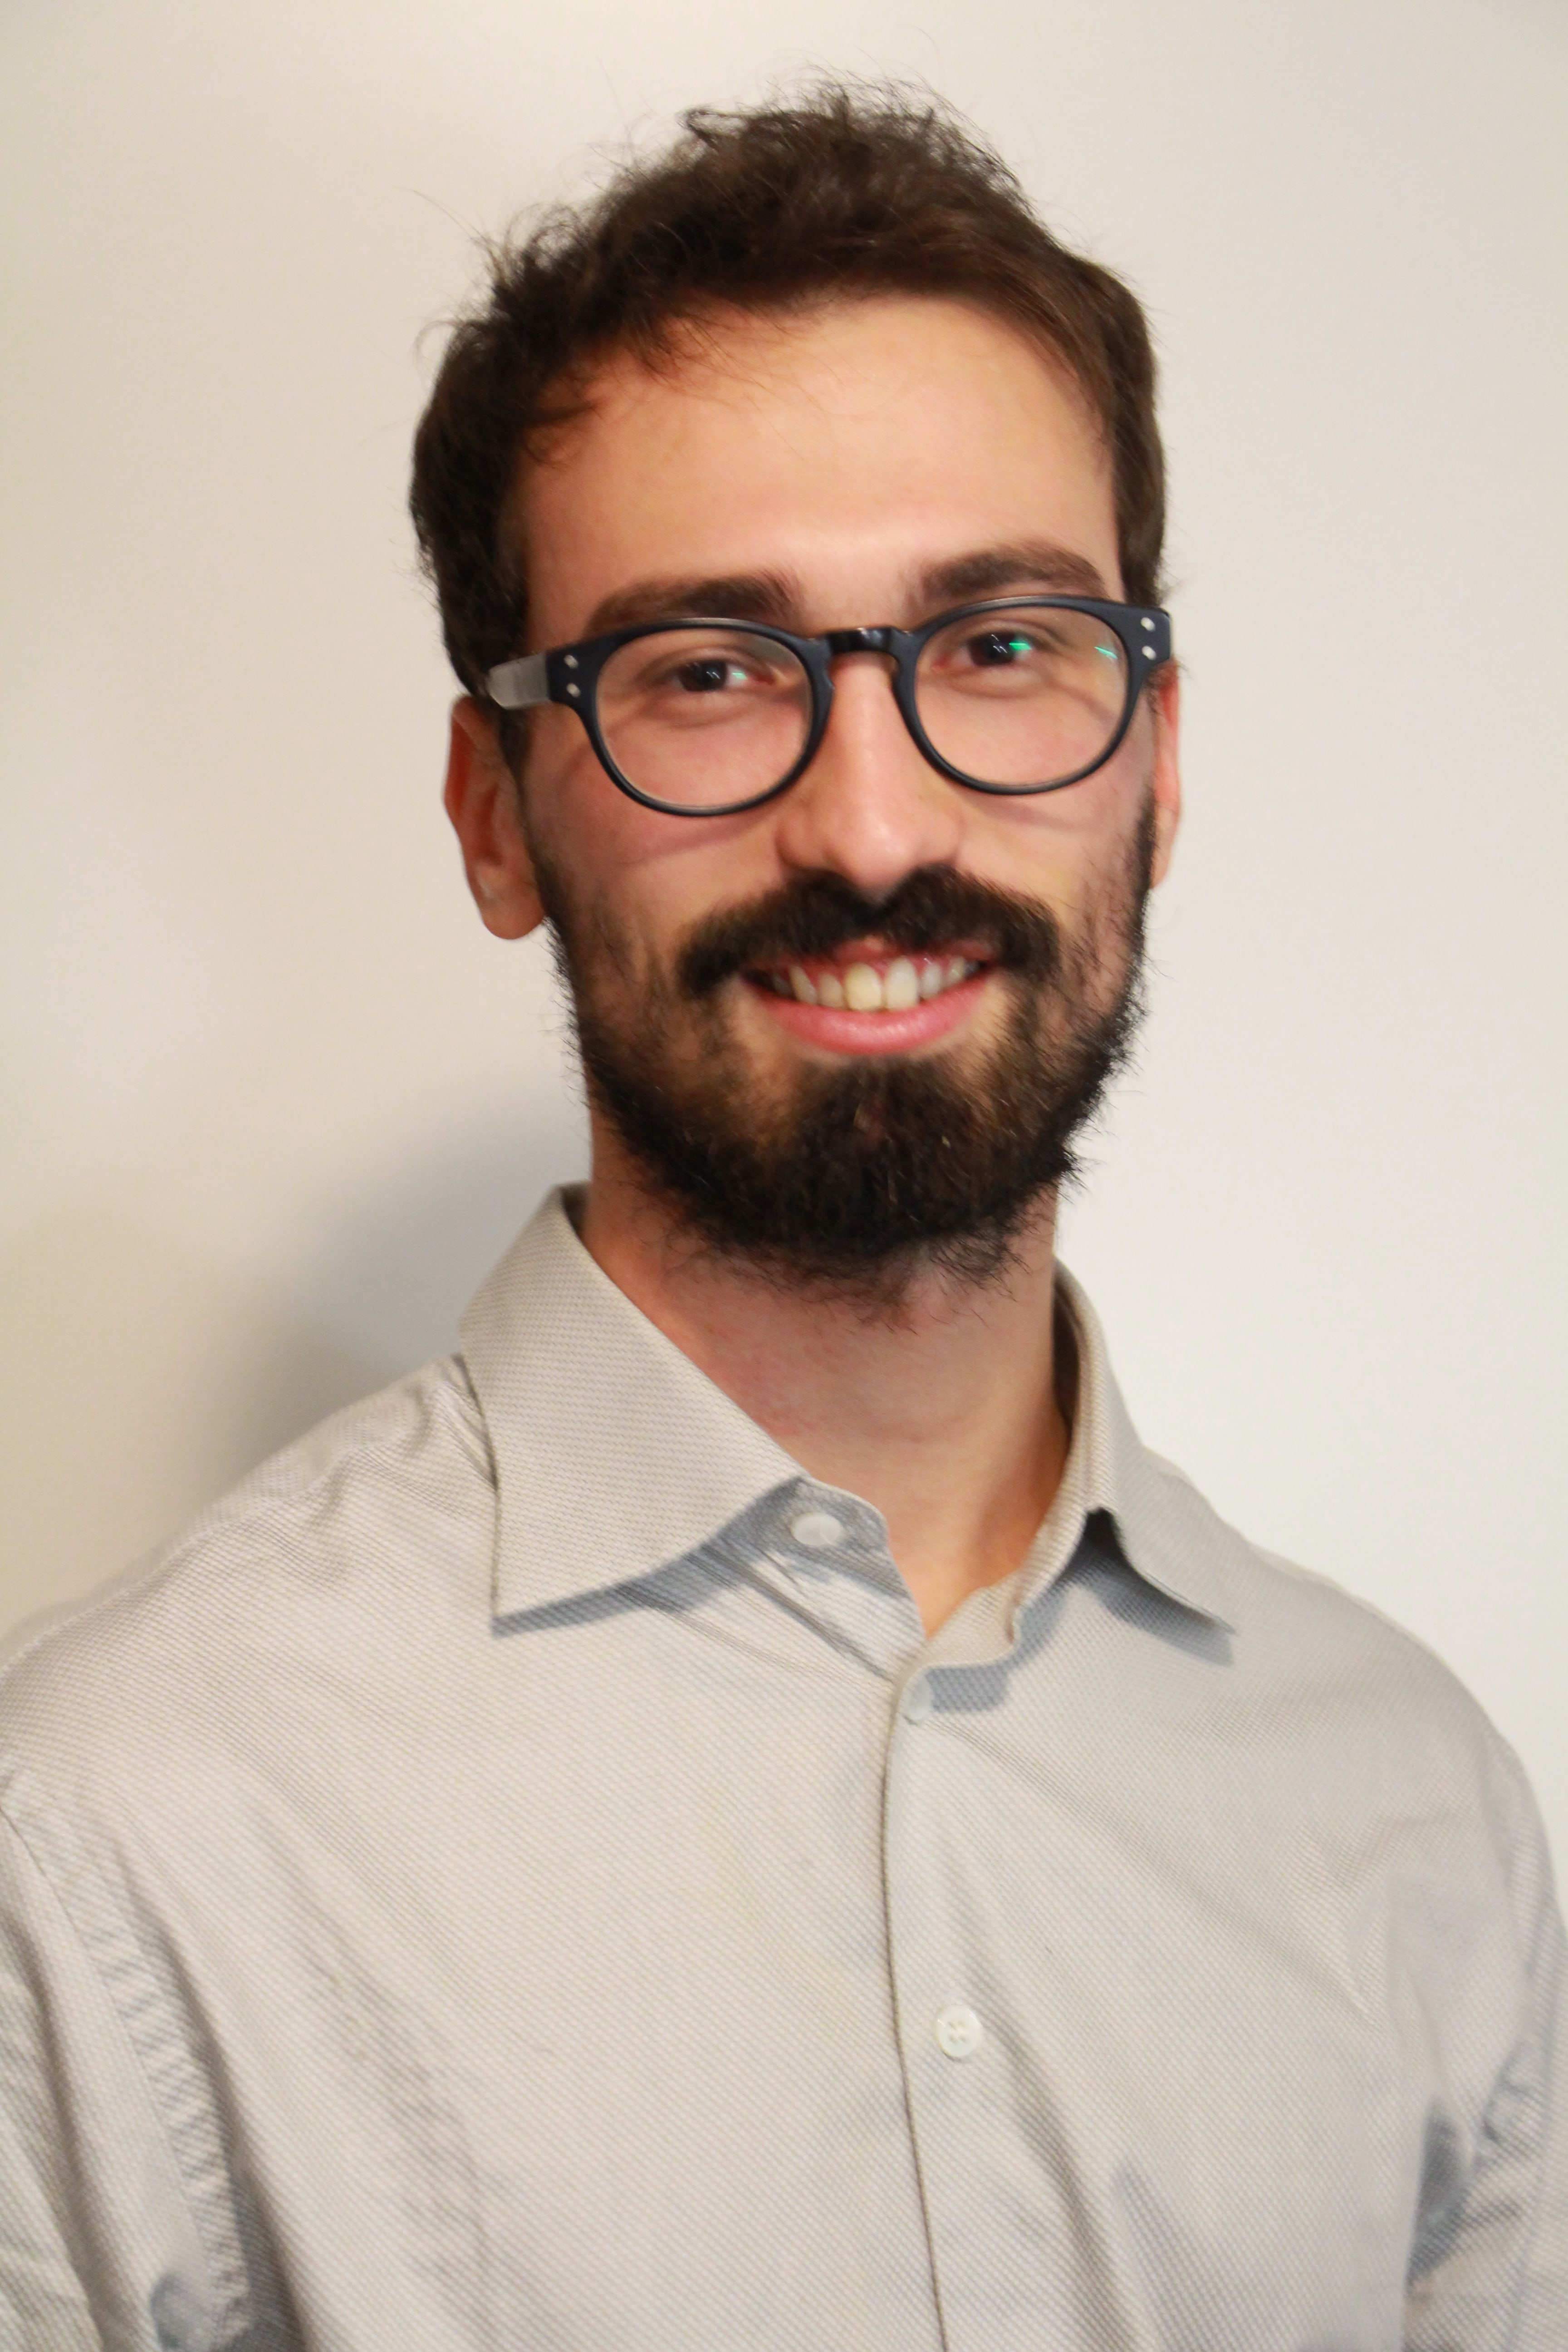
\includegraphics[height=1\linewidth]{Foto_Cv-min.jpg}
\end{center}
\end{minipage}

\vspace{2mm}
%\textbf{\'A la recherche d'une position mois à partir de octobre 2017}
\end{comment}

%----------------------------------------------------------------------------------------
%	EDUCATION SECTION
%----------------------------------------------------------------------------------------


\section{Expériences académiques}
\cventry{Nov. 2020 - Nov. 2022}{Chercheur postdoctoral}{University of Twente}{Enschede, Pays Bas}{}{Méthodes numériques pour problèmes couplés fluide-structure.\\
	Subvention avancée ERC. Chercheur principal: Stefano Stramigioli.}

\section{Formation}

\cventry{2017-2020}{Thèse en Automatique}{ISAE-Supaero}{Toulouse, France}{}{Une formulation port-Hamiltonienne des structures flexibles. Modélisation et discrétisation symplectique par éléments finis. }
% usage: \cventry[spacing]{years}{degree/job title}{institution/employer}{localization}{optionnal: grade/...}{optional: comment/job description}

\cventry{2016--2017}{Master recherche en automatique et traitement d'images}{Université Paris Saclay/\,Supélec}{Paris/Toulouse, France}{}{Modules: identification paramétrique, contrôle avancée des structures flexibles, traitement d'images.}

\cventry{2015--2017}{Double Diplôme en génie aéronautique et aérospatial}{ISAE-Supaero}{Toulouse, France}{}{Spécialisation mathématiques appliques (calcul scientifique) et automatique avancée.}


\cventry{2014--2017}{Master en génie spatial}{Politecnico di Milano}{Milan, Italie}{\textit{110/110 avec mention}}{Modules : Mécanique orbitale, dynamique et contrôle des structures, propulsion thermochimique.}


\cventry{2011--2014}{Licence en génie mécanique}{Politecnico di Milano}{Milan, Italie}{\textit{110/110 avec mention} }{Modules : méthode des éléments finis, vibrations mécaniques, calcul numérique. }

\cventry{2006--2011}{Baccalauréat Littéraire}{Liceo Classico Scipione Maffei}{Verona, Italie}{\textit{100/100}}{}

%\vspace{1mm}

%----------------------------------------------------------------------------------------
%	WORK EXPERIENCE SECTION
%----------------------------------------------------------------------------------------

\section{Expériences}

\cventry{Juillet 2021}{Ecole d'été en intelligence artificielle et apprentissage par renforcement}{Institut CIFAR}{Toronto, Canada}{}{}


\cventry{Janvier 2019, 4 mois}{Chercheur invité}{ITA-Instituto Tecnol\'{o}gico de Aeron\'{a}utica}{S\~{a}o Jos\'{e} dos Campos, Brésil}{}{Collaboration avec Flavio Cardoso-Riberio.}

\cventry{Janvier 2017, 6 mois}{Stage fin études}{CNES-Centre national des études spatiales}{Toulouse}{}{Analyse des débris spatiaux soumis à la pression de radiation solaire.}


%\cventry{2016, 5 mois}{Téléopérations intelligents pour systèmes des micro-drones}{ISAE-Supaero en partenariat avec LAAS}{Toulouse}{}{Codage des lois de commande optimal en C/C++ pour micro-drones engagés en tâches complexes. Équipe de 6 personnes.}

%\cventry{2016, 4 mois}{Dynamique non linéaire des systèmes multi-corps}{ISAE-Supaero}{Toulouse}{}{Modélisation d'une chaîne ouverte des corps en suivant la logique de Simscape Multibody. Validation en Matlab.}

%\cventry{2015, 2 mois}{Transfert interplanétaire}{Politecnico di Milano}{Milan}{}{Étude des trajectoires optimales  avec assistance gravitationnelle pour la minimisation du propergol utilisé. Analyse des perturbations.}

\cventry{2014, 4 mois}{Dynamique d'un manipulateur pour machines de forgeage}{Politecnico di Milano en partenariat avec Danieli S.p.A }{Milan/Buttrio, Italie}{}{Projet sélectionné pour une présentation finale chez \href{https://www.danieli.com/}{Danieli}.}

%\cventry{}{Design d'une éolienne é axe horizontal  }{Politecnico di Milano}{Milano}{}{Dimensionnement général, optimisation performance au point nominal, analyse de performance hors design. équipe de quatre personnes. Publié sur Academia  \textcolor{blue}{\texttt{\href{https://www.academia.edu/9561531/Horizontal_Axis_Wind_Turbine_Design}{Horizontal Axis Wind Turbine Design}}} }

%\cventry{2014, 4 mois}{Analyse é éléments fins d'une pièce mécanique}{Politecnico di Milano}{Milan}{}{Implantation sur Abaqus et codage en Matlab d'un modèle équivalent, validation et comparaison des résultats.}


\section{Activités pédagogiques}
J'ai effectué mes activités d'enseignement à l'Institut Supérieur de l'Aéronautique et de l'Espace, soit pour la formation ingénieur, soit pour les masters internationaux.

\begin{tabular}{p{\dimexpr.15\linewidth-2\tabcolsep}p{\dimexpr.15\linewidth-2\tabcolsep}p{\dimexpr.15\linewidth-2\tabcolsep}p{\dimexpr.4\linewidth-2\tabcolsep}p{\dimexpr.15\linewidth-2\tabcolsep}}
	\hline
	Année & Niveau & Nature  & Discipline & Durée  \\
	\hline
	\multirow{2}{*}{2019-2020} & L1 & TD &  Résolution numérique des EDP & 6h \\
							   & L1 & TD &  Optimisation & 6h \\
	\hline
	\multirow{3}{*}{2018-2019} & L2  & TP-TD  & Automatique & 20h \\
							   & L2  & TD     & Contrôle des structures flexibles & 8h \\
							   & L2  & TP-TD  & Automatic control & 15h \\
	\hline
	\multirow{2}{*}{2017-2018} & L2  & TP-TD  & Automatique & 20h \\
							   & L2  & TP-TD  & Automatic control & 15h \\				   
	\hline
\end{tabular}


\section{Activités scientifiques}

\begin{tabular}{p{\dimexpr.2\linewidth-2\tabcolsep}p{\dimexpr.2\linewidth-2\tabcolsep}p{\dimexpr.6\linewidth-2\tabcolsep}}
	Année & Lieu & Description  \\
	\hline
	2021 & Enschede & Proposition de la thèse "On the modeling and mechanical design of flexures (compliant mechanisms)" entre le département de Robotique et le département d'ingénierie de précision à l'Université de Twente (avec Marijn Nijenhuis). \\
	\hline
	2021  & Berlin & Organisation de la session invitée: "Theoretical and numerical advancements in Hamiltonian formulations of continuum mechanics" pour la conference "Lagrangian and Hamiltonian method in non linear control 2021". \\
	\hline
	2020 & --- & Critiques (Peer reviews) du \textit{Journal of Elasticity}. \\
	\hline
	2019 -2020 & ISAE-Supaero & Organisation et encadrement du Projet Ingénierie et Entreprise intitulé "Simulation et contrôle des structures thermoélastiques pour
	applications spatiales". \\
	\hline
\end{tabular}


\vspace{5mm}

\section{Prix}

\cventry{2021}{Prix de thèse}{Fondation ISAE-SUPAERO}{}{}{}
\cventry{2011-2015}{Dispense des frais de scolarité pour mérite académique.}{Politecnico di Milano}{}{}{}

%----------------------------------------------------------------------------------------
%	LANGUAGES SECTION
%----------------------------------------------------------------------------------------

\vspace{5mm}

\begin{minipage}[t]{0.4\linewidth}
	\section{Langues}
	\cvitem{Anglais}{courant}
	\cvitem{Français}{courant}
	\cvitem{Espagnol}{intermédiaire}
	\cvitem{Portugais}{intermédiaire}
	\cvitem{Italien}{langue maternelle}
\end{minipage}
\begin{minipage}[t]{0.55\linewidth}
	\section{Compétences informatiques}
	\cvitem{Programmes}{Abaqus, Inventor, Solid Works, Labview}
	\cvitem{Langages}{Python (en particulier librairies des éléments finis \firedrake et \fenics), Matlab/Simulink, Java, C, \LaTeX}
\end{minipage}


%----------------------------------------------------------------------------------------
%	COMPUTER SKILLS SECTION
%----------------------------------------------------------------------------------------

%----------------------------------------------------------------------------------------
%	COMMUNICATION SKILLS SECTION
%----------------------------------------------------------------------------------------

% \section{Communication Skills}

% \cvitem{2010}{Oral Presentation at the California Business Conference}
% \cvitem{2009}{Poster at the Annual Business Conference in Oregon}




%\cvitem{Italien}{Langue maternelle}{} \cvitem{Anglais}{Niveau courant : Toeic 965/990 (2014)}{}
%\cvitem{Franéais}{Niveau courant} {} \cvitem{Espagnol}{Niveau débutant} {}

%----------------------------------------------------------------------------------------
%	INTERESTS SECTION
%----------------------------------------------------------------------------------------

\end{document}